% this file is called up by the header file
% content in this file will be fed into the main document
% ----------------------- paths to graphics ------------------------
\graphicspath{{figures/}}

% ----------------------- contents start here ------------------------

\chapter{Model}\label{chap:model}

Hypercube-based NeuroEvolution of Augmenting Topologies (HyperNEAT) is an indirect encoding for evolving artificial neuronal networks (ANNs).

The HyperNEAT algorithm, as illustrated in figure \ref{fig:hyperneat}, consists of three major components:
\begin{enumerate}[(i)]
    \item A Compositional Pattern Producing Network (CPPN) that acts as a genome.
    \item A genetic NEAT algorithm that evolves the CPPN.
    \item An artificial neural network (ANN) that acts as a phenotype.
\end{enumerate}

\begin{figure}[htb]
    \begin{center}
        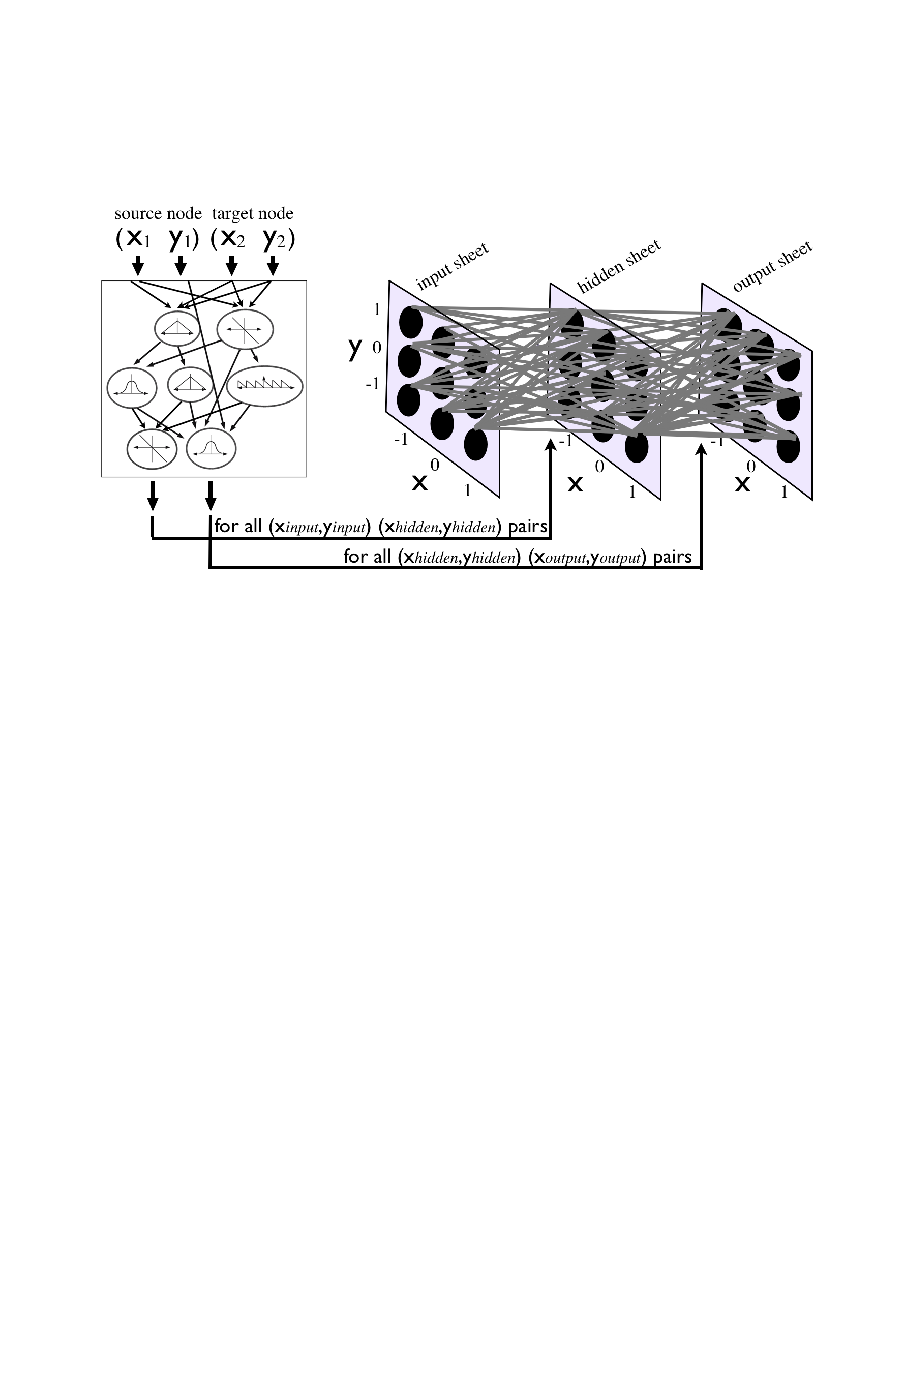
\includegraphics[width=0.9\textwidth]{cppn}
        \caption{Illustration of the HyperNEAT algorithm \cite{clune2011}.
                 A CPPN (left) which is evolved with the NEAT algorithm encodes an ANN (right).}
        \label{fig:hyperneat}
    \end{center}
\end{figure}


